\documentclass[11pt]{beamer}
\usetheme{Madrid}
\usepackage[utf8]{inputenc}

\usepackage[english]{babel}
\usepackage{url}

\usepackage{amsmath}
\usepackage{amsfonts}
\usepackage{amssymb}
\usepackage{graphicx}
\DeclareMathOperator {\argmin}{argmin}

\author{William Grayson Croom}
\title{Classification of Colon/Rectal Tissue}
% Informe o seu email de contato no comando a seguir
% Por exemplo, alcebiades.col@ufes.br
\newcommand{\email}{grayson.croom@gmail.com}
%\setbeamercovered{transparent} 
\setbeamertemplate{navigation symbols}{} 
%\logo{} 
\institute[]{The University of Texas at Dallas \par Mathematical Sciences} 
\date{\today} 
%\subject{}

% ---------------------------------------------------------
% Selecione um estilo de referência
\bibliographystyle{apalike}

%\bibliographystyle{abbrv}
%\setbeamertemplate{bibliography item}{\insertbiblabel}
% ---------------------------------------------------------

% ---------------------------------------------------------
% Incluir os slides nos quais as referências foram citadas
%\usepackage[brazilian,hyperpageref]{backref}

%\renewcommand{\backrefpagesname}{Citado na(s) página(s):~}
%\renewcommand{\backref}{}
%\renewcommand*{\backrefalt}[4]{
%	\ifcase #1 %
%		Nenhuma citação no texto.%
%	\or
%		Citado na página #2.%
%	\else
%		Citado #1 vezes nas páginas #2.%
%	\fi}%
% ---------------------------------------------------------

\begin{document}

\begin{frame}
\titlepage
\end{frame}

\begin{frame}{Summary}
\tableofcontents 
\end{frame}

\section{Introduction to the Problem and Dataset}
    

\begin{frame}{Main Idea}
    The geometric structure of cancerous tissue is very different than that of non-cancerous tissue under a microscope. 
    
    \begin{figure}
        \caption{Cancerous vs Healthy Colon Tissue}
        \label{fig:logo_UFES}
        \centering
        \includegraphics[width=0.5\textwidth]{imagens/cancerous-tissue-image.png}
        
        \medskip
        
        (a) A normal and (b) a cancerous colon tissue image from \cite{tissueImageArticle}. 
    \end{figure}
    
    \vspace{5mm}
    
    Is it possible to use Topological methods to determine whether a tissue sample is cancerous or not?

    \vspace{5mm}
    
\end{frame}

\begin{frame}{The Dataset}
    % \begin{block}{Definition 1.1: Colorectal Histology}
    % The study of the cellular structure of colon and rectal tissue
    % \end{block}
    
    %\vspace{5mm}

    \begin{block}{The Colorectal Histology MNIST}
    A dataset containing 5000 (150x150 pixel) image tiles of colon/rectal tissue, each belonging to 1 of 8 different categories of tissue.
    \end{block}

    \begin{figure}
        \caption{Full Tissue Images}
        \label{fig:logo_UFES}
        \centering
        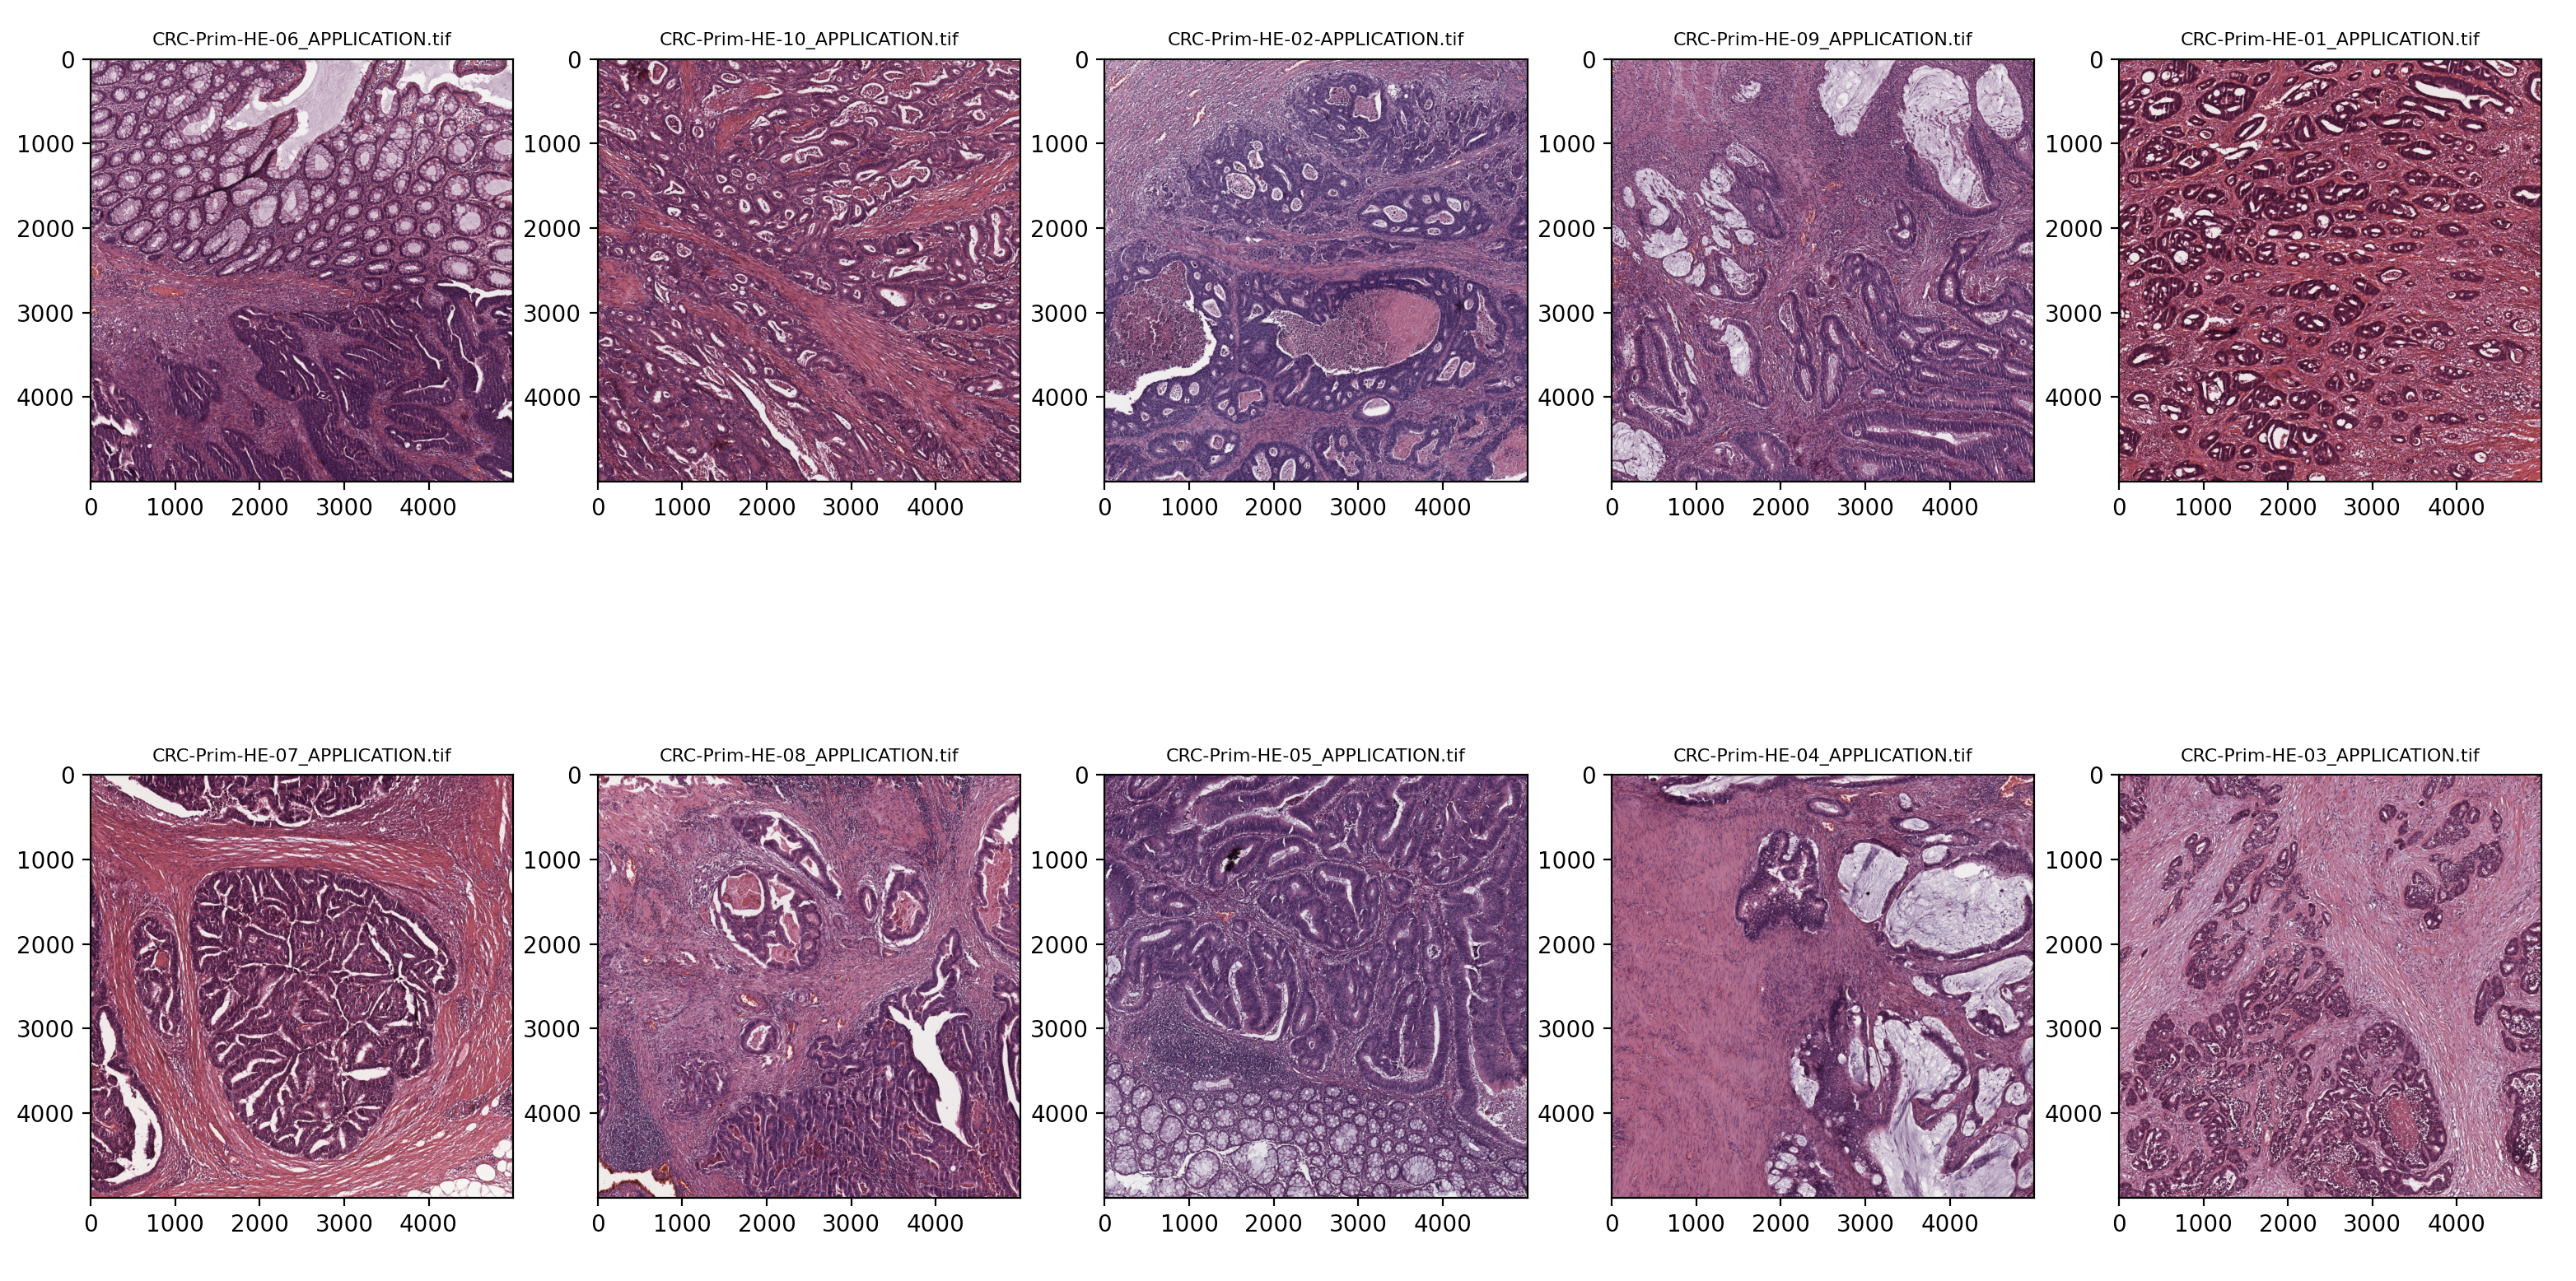
\includegraphics[width=0.5\textwidth]{imagens/dataset_images.png}
        
        \medskip
        
        Figure generated from The Colorectal Histology MNIST dataset \cite{dataset}. 
    \end{figure}
\end{frame}

\begin{frame}{Narrowing the Scope of the Problem}
        
    Classifying the images into 1 of 8 different categories is very complex. For this reason, we will be restricting ourselves to the following 2 settings (as recommended by Dr. Coskunuzer).

    \vspace{5mm}

    The Binary Setting:
    %\begin{block}{The Binary Setting}
    \begin{itemize}
        \item Tissue containing tumors
        \item Complex Stroma tissue 
    \end{itemize}
    %\end{block}

    \vspace{5mm}
    
    The 3-Label Setting:
    %\begin{block}{The 3-Label Setting}
    \begin{itemize}
        \item Tissue containing tumors
        \item Complex Stroma tissue
        \item Tissue containing immune cell conglomerates
    \end{itemize}
    %\end{block}

    

\end{frame}

\begin{frame}{Complex Stroma? Immune Cell Conglomerates?}
    \begin{block}{Definition 1.1: Complex Stroma}
    The cells and tissues that support and give structure to organs, glands, or other tissues in the body. The stroma is mostly made up of connective tissue, blood vessels, lymphatic vessels, and nerves.
    \end{block}
    
    \begin{block}{Definition 1.2: Conglomerate}
    Composed of several parts aggregated into one mass.
    \end{block}

    \begin{block}{Definition 1.3: Immune Cell Conglomerate}
    An aggregated mass of immune cells.
    \end{block}

\end{frame}

\section{Our Approach}

\begin{frame}{Technical Outline}
    When beginning the project, I needed to figure out how the program would look at a high level.
    
    \vspace{4mm}
    
    The following is how I decided data would flow through the program:
    \begin{enumerate}
        \item Import all images from dataset into my program, probably as numpy arrays.
        \item Transform the images in some way to make them easier to process.
        \item Generate complexes of the data based on a filtration function.
        \item Create persistence diagrams and obtain betti-0/betti-1 lifetimes of the topological objects in my cancer images.
        \item Vectorize those lifetimes to make this important topological data discrete.
        \item Do a 80:20 split of these vectors for training and testing, respectively.
        \item Train both a Random Forest Classifier and a Gradient Boosting Classifier on the vectorized lifetimes and see which performed better.
    \end{enumerate}
\end{frame}

\begin{frame}{The Structure of Our Dataset}
    \begin{figure}
        \caption{Directory Structure of Colorectal Histology MNIST dataset}
        \centering
        \includegraphics[width=0.55\textwidth]{imagens/dataset_directory_structure.png}

        Note: there are 300-800 tissue tif images under each numbered directory
    \end{figure}
\end{frame}

\begin{frame}{Getting Our Dataset into Python!}
    My strategy for importing this dataset into my program is:
    \begin{enumerate}
        \item First I pulled all directory names from the dataset into python.
        \item Next I checked to see if the directory name matched the 3 labels I was going to be training the models on.
        \item Finally I read all the images belonging to these selected directories into python using the PIL Image library.
        \item As they were being read into python, they would be placed into the appropriate "setting" array (i.e. binary or 3-label)
    \end{enumerate}

    \vspace{3mm}

    \par I wanted the process of importing data to be general enough such that one could easily change which labels are important to the program. This sacrifices some efficiency, but this generally isn't an issue as this process never takes more than a few seconds.
\end{frame}

\begin{frame}{Image Transformations Applied}
    The first thing I did was gray-scale the images.
    
    \vspace{3mm}
    
    Then, I reduced their size to 28x28 pixels since originally they were 150x150 pixels.
    
    \vspace{3mm}

    Finally, the PIL images were converted to NumPy arrays since they are easier to work with, in a data science setting.
    
    \vspace{3mm}
    
    \begin{block}{Note}
        Later on, I would come back and change this resize to 75x75 pixels, because after extensive testing I found I couldn't reduce the images further without significantly reducing the accuracy of my models. I had originally thought that 28x28 pixels would be sufficient since other machine learning models that don't utilize topological methods were able to get good results with these small images, but this was not the case when training the models on the topological data of the images.
    \end{block}
    
\end{frame}

\begin{frame}{First Approach to the Vectorization Pipeline}
    \par Finally, it was time to convert the possibly cancerous tissue images into vectors that could be consumed by my models.
    
    \vspace{3mm}
    
    \par The first pipeline I considered was the following:
    
    \begin{enumerate}
        \item Convert image into point-cloud data
        \item Obtain Persistence Diagrams from Vietoris-Rips filtrations
        \item Vectorize betti-0 and betti-1 lifetimes
    \end{enumerate}
    
    \vspace{3mm}
    
    \par However, no matter what vectorization methods were used (diagram.Amplitude, diagram.PersistenceEntropy, diagram.NumberOfPoints), both the Random Forest Classifier and the Gradient Boosting Classifier performed poorly.
    
    \vspace{3mm}
    
    \par It seemed like the conversion from image data to point-cloud data wouldn't work for my purposes. I would have to try something else.
\end{frame}

\begin{frame}{A Better Approach}
    \par The vectorization pipeline I landed on after extensive testing is:
    \begin{enumerate}
        \item Create Persistence diagrams of the lifetimes of cubical complexes of homology dimension-0 (holes) and dimesion-1 (loops).
        \item Apply Linear Scaler to diagrams (this doesn't matter as much without the density filtration).
        \item Create a vector of the amplitudes of our generated lifetimes using a "persistence image" metric.
    \end{enumerate}
    
    \begin{figure}
        \caption{Code to create our Sklearn pipeline}
        %\label{fig:logo_UFES}
        \centering
        \includegraphics[width=0.8\textwidth]{imagens/pipeline_code.png}
    \end{figure}
    
\end{frame}

\begin{frame}{Notes on This Approach}
    \begin{block}{Sidenote}
    At first I tried applying a Density Filtration to my images before generating persistence diagrams from cubical complexes, but these performed much worse than directly generating persistence diagrams from the gray-scaled image.
    \end{block}

    \vspace{7mm}

    \par Intuitively, this makes sense, since cancerous cells nearly always look "deformed" from a geometric point of view, whereas cancerous tissue is only higher density after a lot of time and when confined in a membrane preventing it from replicating outwards.
\end{frame}

\begin{frame}{Linearly Scaled Persistence Diagrams}
    \begin{figure}
        \caption{Linearly Scaled Persistence Diagrams}
        \centering
        \includegraphics[width=0.5\textwidth]{imagens/persistence_diagrams.png}
        
        \medskip
        
    \end{figure}
\end{frame}

\begin{frame}{The Vectorization Process}
    \par Finally, we want to make our continuous persistence diagram discrete without losing too much information.
    \vspace{3mm}
    \par In the end, I decided to use an Amplitude transformer from the Giotto-TDA library. This transformer:
    \begin{enumerate}
        \item Takes in persistence diagrams
        \item For each point in each diagram, calculate the amplitude of the point using a predetermined metric.
        \item Collect each of these points' amplitude into a vector
        \item Collect each of these vectors into a NumPy array.
    \end{enumerate}
    
    \vspace{2mm}

    \par I used a built-in metric called the \textit{persistence image metric}, which is a distance between Gaussian-smoothed diagrams represented on birth-persistence axes \cite{persistenceImageMetric}. My rationale for using it instead of the Bottleneck or Wasserstein metrics was purely empirical, namely, this metric far outperformed all other built-in metrics by more than 10 percent after training the models on the produced vectors.

\end{frame}

\begin{frame}{Why Random Forest? Why Gradient Boosting?}
    First, it's important to understand that while we informally refer to the RandomForestClassifier and GradientBoostingClassifier as "models", they are actually a collection of models called \textbf{ensembles}.

    \vspace{3mm}
    
    \begin{block}{Definition 3.1: Ensemble }
    The goal of [ensembles] is to combine the predictions of several base estimators built with a given learning algorithm in order to improve generalizability/robustness over a single estimator. 
    \end{block}

    \vspace{3mm}

    There are two types of ensembles, namely:
    \begin{enumerate}
        \item \textit{averaging ensembles} - independent estimators with averaged results
        \item \textit{boosting ensembles} - sequential estimators each tasked with reducing the bias of the previous estimator
    \end{enumerate}

    \vspace{5mm}

    
    Information from Sklearn \cite{ensembleInfo}
\end{frame}

\begin{frame}{Hyperparameter Selection}
    \begin{block}{What is a hyperparameter?}
    In machine learning, a hyperparameter is a parameter whose value is used to control the learning process. By contrast, the values of other parameters (typically node weights) are derived via training. \cite{hyperparam}
    \end{block}

    \vspace{3mm}

    \par In other words, a hyperparameter is a variable that affects the process by which the model learns.
    
    \vspace{3mm}
    
    \par For example: When constructing a Sklearn RandomForestClassifier object, you can pass it an argument of "max\_depth" and "n\_estimators" which changes the maximum depth of every tree as well as the number of trees in our forest, respectively.
    
    \vspace{3mm}
    
    \par Without the ability to tune hyperparameters, we can't be sure our model wouldn't have performed better than with shallower trees.
    
    \vspace{3mm}
\end{frame}

\begin{frame}{Important Hyperparameters}
    For the Random Forest Model, we'd like to tune:
    \begin{itemize}
        \item \textit{max\_depth} - Maximum depth of each tree. 
        \item \textit{n\_estimators} - Number of trees in our decision forest.
    \end{itemize}
    
    \vspace{5mm}
    
    For the Gradient Boosting Model, we'd like to tune all the same parameters with the addition of:
    \begin{itemize}
        \item \textit{learning\_rate} - Changes the amount each tree "contributes" to the overall classification.
    \end{itemize}

    \begin{block}{Note}
        The higher the \textit{learning\_rate}, the lower the contribution each tree has to the final classification.
        There is a trade-off between \textit{learning\_rate} and \textit{n\_estimators} \cite{gradientboostdocs}
    \end{block}
\end{frame}

\begin{frame}{Hyperparameter Tuning In Context}
    \par Now obviously these parameters can be manually tuned, but in order to ensure the best results we want the program to find the best parameters from a list of reasonably selected parameters.
    
    \vspace{3mm}
    
    \par Luckily, Sklearn has a built-in feature called GridSearchCV (CV stands for cross-validation), which takes in a list of reasonable parameters and finds the parameters that maximize the accuracy of your model.
    
    \vspace{3mm}
    
    \par In my program, models are only trained after the ideal hyperparameters are found for each setting/model.
    
    \begin{figure}
        \caption{Simple function to apply GridSearchCV to a given model}
        \label{fig:logo_UFES}
        \centering
        \includegraphics[width=0.7\textwidth]{imagens/grid_search_fn.png}
        
        \medskip
    \end{figure}
\end{frame}

\begin{frame}{Other Cool Features Included in Program}
    Some nice features I included:
    \begin{itemize}
        \item The ability to save trained models to disk.
        \item The ability to import previously trained models from disk into the program.
        \item The ability to generate/display the diagrams and images used in this presentation.
    \end{itemize}

    \vspace{3mm}

    \par One thing I kept finding myself needing to do was function composition, something rather annoying to do in languages without function currying. I couldn't find a standard library implementation of this basic feature, but luckily I found this nifty implementation online.

    \begin{figure}
        \caption{Python Function Composition}
        \centering
        \includegraphics[width=0.65\textwidth]{imagens/function_composition.png}

    \end{figure}
    
\end{frame}

\section{Results}

\begin{frame}{Example Program Output}
    \par \centering Finally, after many adjustments, our program works!
    \begin{figure}
        \caption{Output of Model Training}
        \centering
        \includegraphics[width=0.37\textwidth]{imagens/small_program_output.png}

    \end{figure}
\end{frame}

\begin{frame}{Results}
    \begin{table}
        \caption{Binary Setting}
        \label{tab:modelo_tabela}
        \centering
        \begin{tabular}{|c|c|c|}
	    \hline
	    \textbf{Method} & \textbf{Model Score} & \textbf{AUC ROC} \\ \hline
	    Random Forest & 0.858333 & 0.8980555  \\ \hline
	    Gradient Boosting & 0.8666 & 0.9108333   \\ \hline
        \end{tabular}
        
        \medskip
    \end{table}

    \begin{table}
        \caption{3-Label Setting}
        \label{tab:modelo_tabela}
        \centering
        \begin{tabular}{|c|c|c|}
	    \hline
            \textbf{Method} & \textbf{Model Score} & \textbf{TP, TN, FN, FP} \\ \hline
            Random Forest & 0.7111 & 24, 17, 11, 2    \\ \hline
            Gradient Boosting & 0.7 & 25, 17, 10, 2  \\ \hline
        \end{tabular}
        
        \medskip
    \end{table}
\end{frame}

\begin{frame}{Known Results}
    \begin{figure}
        \caption{Known Results}
 
        \centering
        \includegraphics[width=1\textwidth]{imagens/known_results.png}
        
        \medskip

        Data provided by \cite{knownresults}
    \end{figure}
\end{frame}

\begin{frame}{Thoughts on Results}
    \par The areas under the binary setting ROC curve are around 0.9, which leads me to believe it's highly likely the displayed scores accurately represent the prediction power of my models in general.
    
    \vspace{3mm}
    
    \par Also, after running a few times it seems like the Random Forest model is better in the binary setting whereas the gradient-boosted decision tree model works better in the 3-label setting.
    
    \vspace{3mm}
    
    \par Something I don't like about my 3-label results is how my models tend towards false negatives in the case that they fail. This is a big issue in a clinical setting as we'd rather spend the resources to perform tests on a patient that doesn't have cancer than have patients with cancer slip through the cracks. However, there could be contexts where we want to be very certain we only get images with cancer, in these contexts we'd prefer false negatives to false positives.
\end{frame}

\section{Conclusion}

\begin{frame}{Final Thoughts and Conclusion}
    \par One area I could try to explore to increase the accuracy of classification is creating my own ensembles. Currently, the program trains 2 ensembles that are provided by Sklearn, but I'm sure some data exploration could lead to some insights as to how these ensembles could be redesigned.

    \vspace{8mm}

    \par So to conclude, I'd like my 3-Label setting accuracy to be a bit better. However, I'm fairly happy with these results overall, especially with my accuracy in the binary setting.
\end{frame}

\section{References}
\begin{frame}[shrink=15]{References}
    \bibliography{referencias}
\end{frame}

\begin{frame}

\begin{center}
    Thanks!
    
    \email
\end{center}

\begin{figure}
    \centering
    \includegraphics[width=0.3\textwidth]{imagens/utd.png}
\end{figure}

\end{frame}

\end{document}